\section{Method}
\subsection{System overview}

%TODO: add figure of system diagram (FSM + RAM):
\begin{figure}
    \centering
    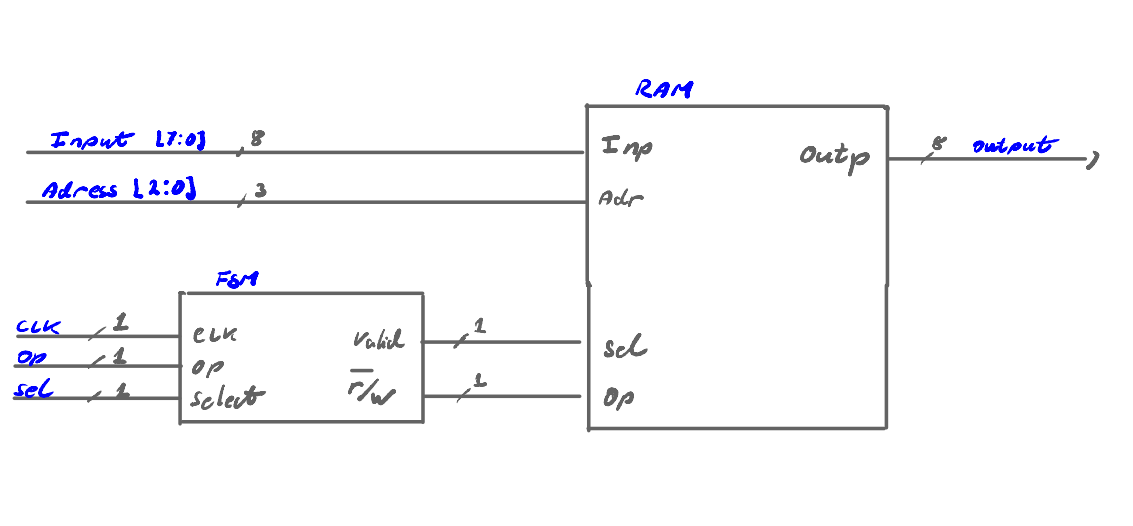
\includegraphics[width=0.8\linewidth]{LaTeX_2/Figures/memory_block_schematic.png}
    \caption{System diagram}
    \label{fig:03:system_diagram}
\end{figure}

Our system consists of a Finite State Machine and a Random Access Memory, as can be seen in \autoref{fig:03:system_diagram}. The FSM serves as a control unit to make sure all operations on the RAM are performed in a stable manner. The FSM is connected to a clock signal, but the RAM is not directly, only indirectly through controll by the FSM.

%%%%%%%%%%%%%%%%%%%%%%%%%%%%%%%%%%%%%%%%%%%%%%%%%%%%%%%%%%%%%%%%%%%%%%%%%%%%%%%%%%%%%%%%%%%%%
%                                         RAM                                               %
%%%%%%%%%%%%%%%%%%%%%%%%%%%%%%%%%%%%%%%%%%%%%%%%%%%%%%%%%%%%%%%%%%%%%%%%%%%%%%%%%%%%%%%%%%%%%
\subsection{RAM}
The RAM subsystem consists of eight bitcells forming eight bytecells that stack on top of each other to form the full memory. It has these inputs and outputs:
\begin{itemize}
    \item \makebox[2cm]{adr \hfill} - 3-bit address signal
    \item \makebox[2cm]{inp \hfill} - 8-bit input data to be stored in address
    \item \makebox[2cm]{outp \hfill} - 8-bit output data to be read from address
    \item \makebox[2cm]{op \hfill} - either 0 for read or 1 for write
    \item \makebox[2cm]{sel \hfill} - must be 1 for op to affect the circuit
\end{itemize}

When the circuit is reading, meaning \textsc{op} is low, the output is what is stored in the currently addressed bytecell. When it is writing, the outp is Z (high resistance), meaning it can be easily overwritten, and should not be trusted. We chose our output to be Z as that seemed like the clearest solution, since it is necessary for the circuit to be in read mode in order to be read from.

The RAM's circuit is as in \autoref{fig:03:RAM_schematic}. It consists of eight bytecell modules. Each of the output busses is connected together as it is only possible to read from one of the bytecell modules at a time.

\begin{figure}
    \centering
    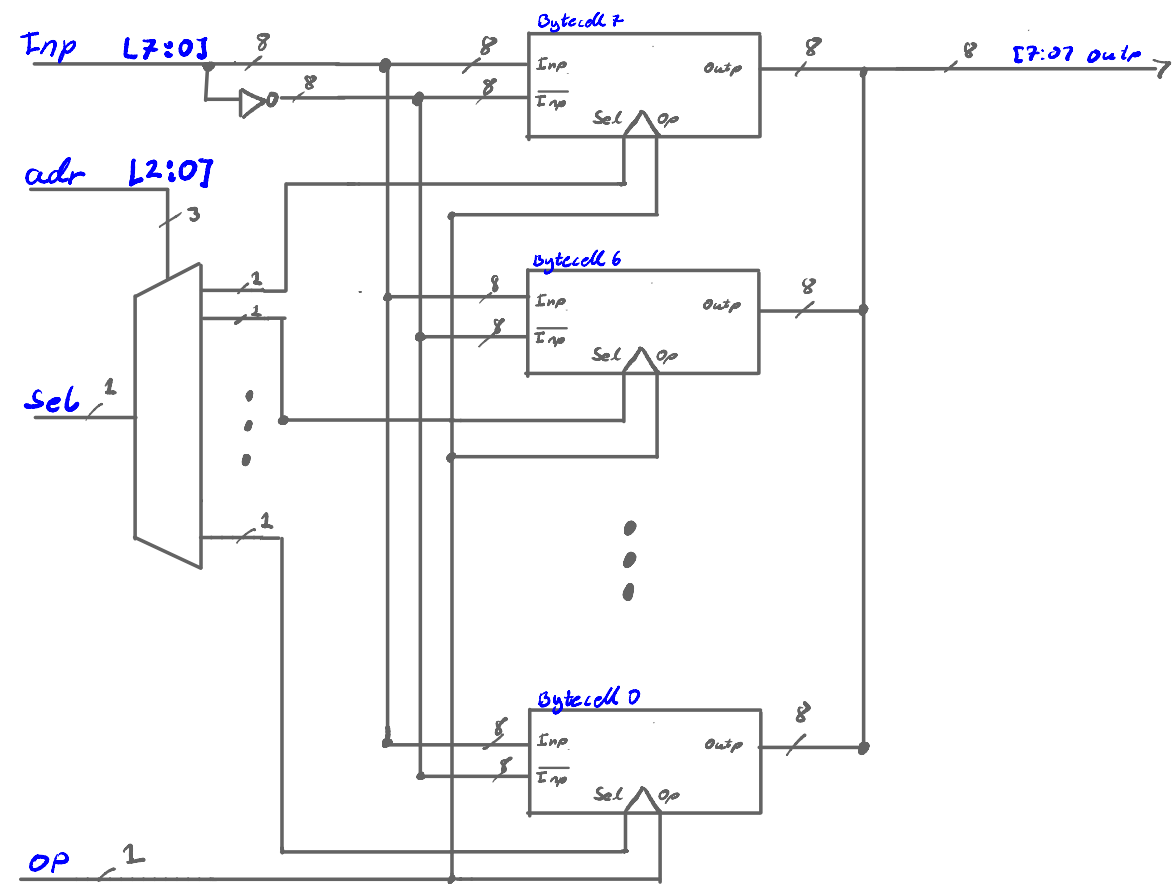
\includegraphics[width=0.8\linewidth]{LaTeX_2/Figures/ram_schematic.png}
    \caption{Full schematic for the RAM subsystem}
    \label{fig:03:RAM_schematic}
\end{figure}


%%%%%%%%%%%%%%%%%%%%%%%%%%%%%%%%%%%%%%%%%%%%%%%%%%%%%%%%%%%%%%%%%%%%%%%%%%%%%%%%%%%%%%%%%%%%%
%                                         BITCELL                                           %
%%%%%%%%%%%%%%%%%%%%%%%%%%%%%%%%%%%%%%%%%%%%%%%%%%%%%%%%%%%%%%%%%%%%%%%%%%%%%%%%%%%%%%%%%%%%%
\subsubsection{The bitcell}
The bitcell concists of a D-latch and a tri-state-buffer. The logic schematic of the D-latch, connected to the transistor schematic of a tri-state-buffer, can be seen in \autoref{fig:03:bitcell_schematic}.

\begin{figure}[H]
    \centering
    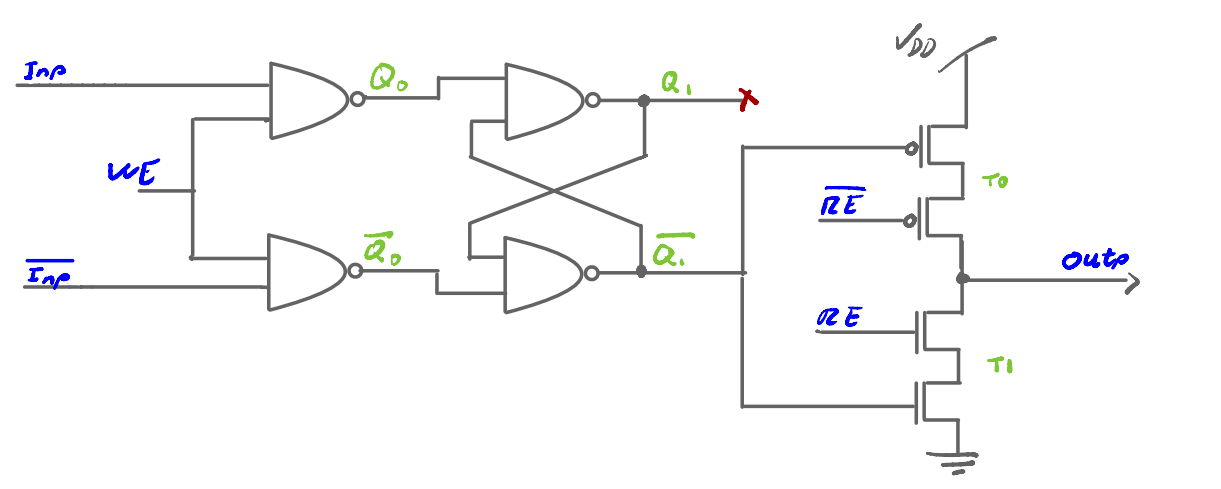
\includegraphics[width=0.8\linewidth]{LaTeX_2/Figures/bitcell_schematic.png}
    \caption{Wiring schematic for the bitcell module}
    \label{fig:03:bitcell_schematic}
\end{figure}

The bitcell has inputs and outputs:
\begin{itemize}
    \item \makebox[2cm]{inp \hfill} - The input bit to be stored
    \item \makebox[2cm]{inpn \hfill} - (input not) The inverse of the input bit
    \item \makebox[2cm]{outp \hfill} - The output when the circuit is read
    \item \makebox[2cm]{WE \hfill} - Write Enable, must be high to store a new value
    \item \makebox[2cm]{RE \hfill} - Read Enable, must be high to set outp to the stored value
\end{itemize}

The stored value sits in $\overline{Q_1}$, since the tri-state buffer acts as an iverter. We choose to implement the bitcell with a tri-state-buffer in order to make the output high impedance ($Z$) when \textsc{RE} is low. This is to ensure that the common bus in the RAM module can be overwritten by the selected bytecell module if \textsc{RE} is active.
This simplifies the rest of the design, since there is no need for a multiplexer to choose which address to read data from. 

\hspace{}

The leakage current of each bitcell are a sum of the leakage current of all the transistors that make up one bitcell. In total there are 20 transistors in each bitcell, 10 \textsc{NMOS} and 10 \textsc{PMOS}. The leakage current of one \textsc{NMOS} can be estimated from equation \ref{eq:03:leakage_current}
TODO: Bitcell analog properties. W, L, VDD




%%%%%%%%%%%%%%%%%%%%%%%%%%%%%%%%%%%%%%%%%%%%%%%%%%%%%%%%%%%%%%%%%%%%%%%%%%%%%%%%%%%%%%%%%%%%%
%                                         BYTECELL                                          %
%%%%%%%%%%%%%%%%%%%%%%%%%%%%%%%%%%%%%%%%%%%%%%%%%%%%%%%%%%%%%%%%%%%%%%%%%%%%%%%%%%%%%%%%%%%%%
\subsubsection{The bytecell}
The bytecell consists of 8 bitcells and an F-block (function block) meant to translate the input signals of the bytecell to the required inputs of each of its bitcells. The bitcells all write their outputs to 8 different wires, which we refer to as the data bus. The bytecell can be seen in \autoref{fig:03:bytecell_schematic}.

\begin{figure}[H]
    \centering
    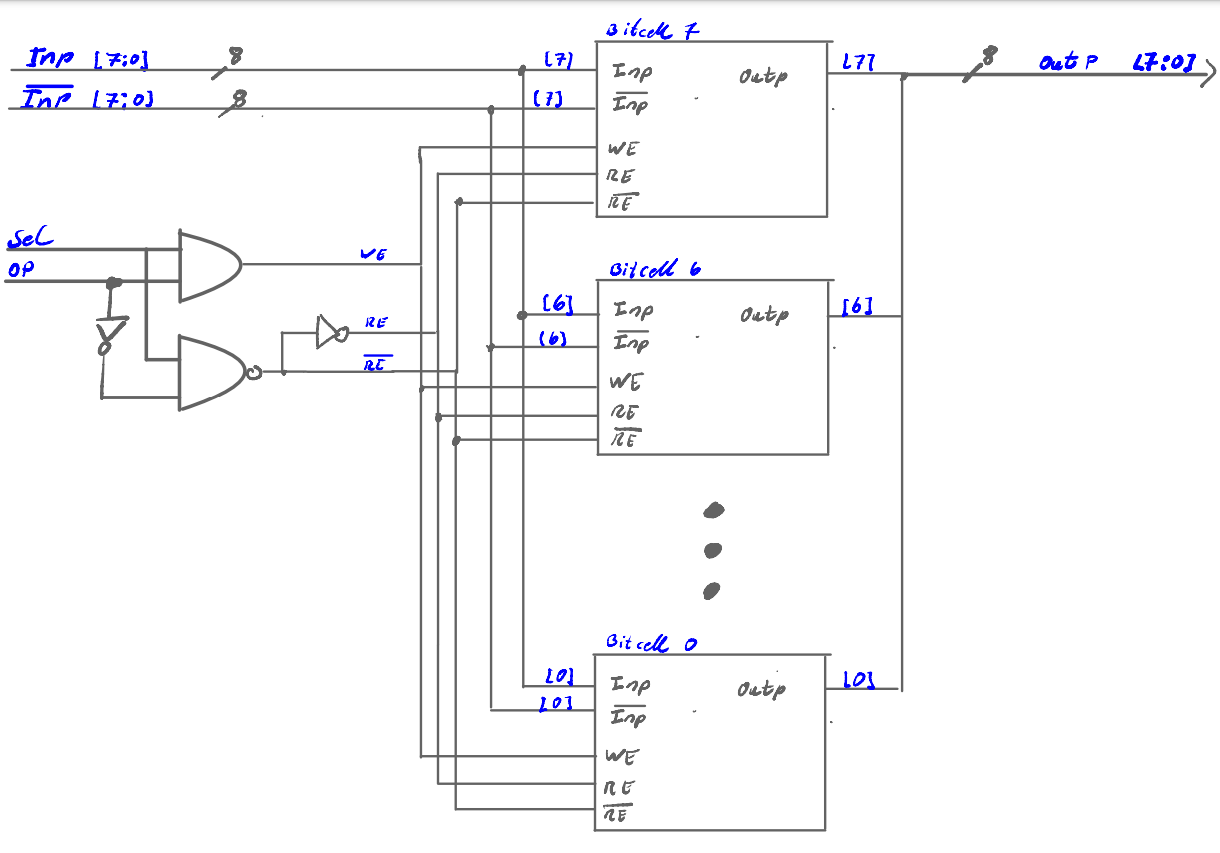
\includegraphics[width=0.8\linewidth]{LaTeX_2/Figures/bytecell_schematic.png}
    \caption{Wiring schematic for the bytecell module}
    \label{fig:03:bytecell_schematic}
\end{figure}

The inputs and outputs of the bytecell are almost identical to those of the RAM, with the exception of there being no address signal, and the input having to be written both normally and inverted. Having the inverse signal at this level means saving transistors, as there will be one inverter for each of the 8 data bus wires one level higher, instead of one inverter for every bitcell.

The F-block was designed to set WE high only when op and sel are high, and to set RE high only when op is low and sel is high, and otherwise to set both WE and RE to low.


%%%%%%%%%%%%%%%%%%%%%%%%%%%%%%%%%%%%%%%%%%%%%%%%%%%%%%%%%%%%%%%%%%%%%%%%%%%%%%%%%%%%%%%%%%%%%
%                                         FMS                                               %
%%%%%%%%%%%%%%%%%%%%%%%%%%%%%%%%%%%%%%%%%%%%%%%%%%%%%%%%%%%%%%%%%%%%%%%%%%%%%%%%%%%%%%%%%%%%%
\subsection{FSM}
The finite state machine is meant to work as an interface for stable use of the RAM subsystem. Together they make up the memory system. It was designed by looking at the state diagram, \autoref{fig:03:state_diagram}, from the project task. Then proceeding by giving code values to each of the states, \autoref{tab:03:state_code}, setting up a truth table, \autoref{tab:03:FSM_truth_table}, and using the logical relations between the inputs, outputs, current state and next state, \autoref{eq:03:boolean_equation}, to design a typical FSM circuit, \autoref{fig:03:FSM_schematic}.


The transistor circuit implementation of the D-latch in the bitcell can be seen in \autoref{fig:03:D-latch_schematic}.

%TODO: add figure of transistor circuit for the D-latch
\begin{figure}[H]
    \centering
    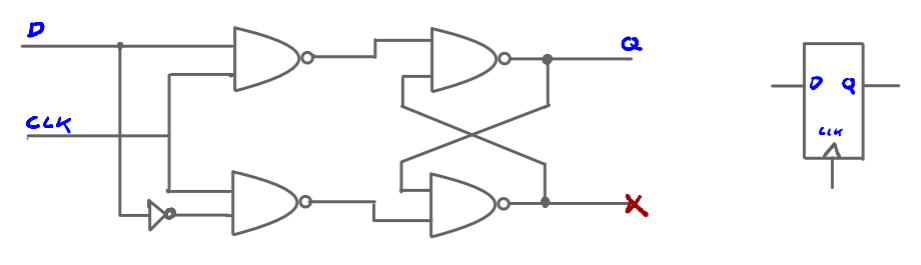
\includegraphics[width=0.8\linewidth]{LaTeX_2/Figures/flipflop.png}
    \caption{Circuit schematic of the D-latch in the bitcell}
    \label{fig:03:D-latch_schematic}
\end{figure}


\begin{figure}
    \centering
    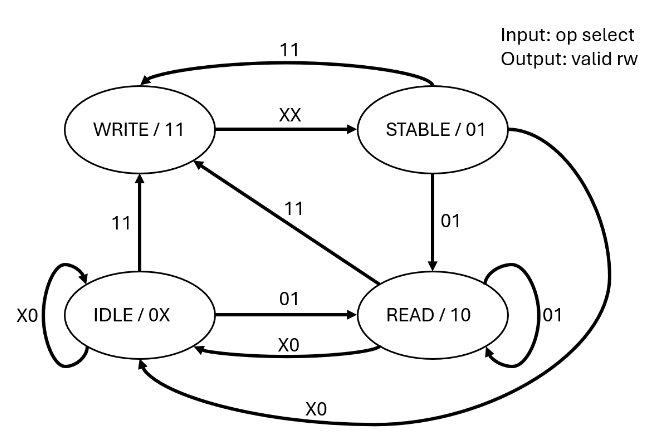
\includegraphics[width=0.8\linewidth]{LaTeX_2/Figures/state_diagram.png}
    \caption{Desired state diagram \cite{oppgavebeskrivelse}}
    \label{fig:03:state_diagram}
\end{figure}

\begin{table}[]
    \caption{State code and their meaning.}
    \centering
    \begin{tabular}{|l|c|}
        \hline
        State   &   Code    \\  \hline
        IDLE    &   0 X     \\  
        STABLE  &   0 1     \\
        READ    &   1 0     \\
        WRITE   &   1 1     \\  \hline
    \end{tabular}
    \label{tab:03:state_code}
\end{table}

\subsubsection{Circuit design}
\begin{figure}
    \centering
    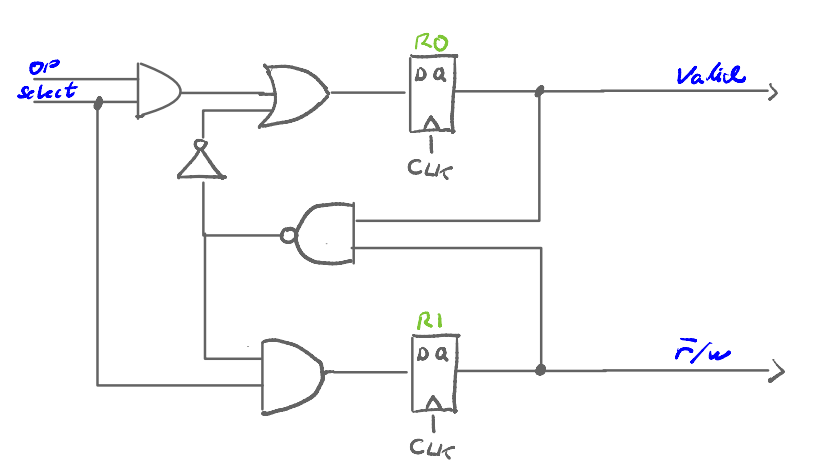
\includegraphics[width=0.8\linewidth]{LaTeX_2/Figures/fsm_schematic.png}
    \caption{Wiring schematic for the FSM logic.}
    \label{fig:03:FSM_schematic}
\end{figure}

\begin{table}[]
    \caption{Truth table for Finite State Machine.}
    \centering
    \begin{tabular}{|cc|cc|cc|cc|}
        \hline
        \multicolumn{2}{|l|}{State} & \multicolumn{2}{l|}{Input} & \multicolumn{2}{l|}{State nxt} & \multicolumn{2}{l|}{Output}        \\ \hline
                     &              & Op          & Sel          &                &               & Valid & R/W \\
        A            & B            & C           & D            & E              & F             & G     & H                          \\ \hline
        0            & 0            & 0           & 0            & 0              & X             & 0     & X                          \\
        0            & 0            & 0           & 1            & 1              & 0             & 0     & X                          \\
        0            & 0            & 1           & 0            & 0              & X             & 0     & X                          \\
        0            & 0            & 1           & 1            & 1              & 1             & 0     & X                          \\
        0            & 1            & 0           & 0            & 0              & X             & 1     & 0                          \\
        0            & 1            & 0           & 1            & 1              & 0             & 1     & 0                          \\
        0            & 1            & 1           & 0            & 0              & X             & 1     & 0                          \\
        0            & 1            & 1           & 1            & 1              & 1             & 1     & 0                          \\
        1            & 0            & 0           & 0            & 0              & X             & 0     & 1                          \\
        1            & 0            & 0           & 1            & 1              & 0             & 0     & 1                          \\
        1            & 0            & 1           & 0            & 0              & X             & 0     & 1                          \\
        1            & 0            & 1           & 1            & 1              & 1             & 0     & 1                          \\
        1            & 1            & 0           & 0            & 0              & 1             & 1     & 1                          \\
        1            & 1            & 0           & 1            & 0              & 1             & 1     & 1                          \\
        1            & 1            & 1           & 0            & 0              & 1             & 1     & 1                          \\
        1            & 1            & 1           & 1            & 0              & 1             & 1     & 1                          \\ \hline
    \end{tabular}
    \label{tab:03:FSM_truth_table}
\end{table}



\begin{equation}
\begin{split}
    E   &=  D \cdot \overline{A \cdot B}\\
    F   &=  A \cdot B + C \cdot D       \\
    G   &=  B                           \\
    H   &=  A
\end{split}
    \label{eq:03:boolean_equation}
\end{equation}

